\section{Related Work}
\label{sec:related_work}



Encrypted traffic classification has evolved substantially over the past decade, transitioning from traditional port-based heuristics toward data-driven deep learning approaches. The widespread adoption of encryption protocols and tunneling mechanisms, particularly Virtual Private Networks (VPNs), has rendered signature-based inspection and port-based identification increasingly ineffective. Consequently, modern research focuses on learning discriminative representations directly from traffic data. Nevertheless, two fundamental challenges remain: the scarcity of labeled datasets and the difficulty of effectively integrating heterogeneous traffic representations such as raw payloads and flow-level statistics. Table \ref{tab:rw_comparison} summarizes the key differences between existing frameworks and the proposed LE-MVCL approach.

Early deep learning methods demonstrated that raw packet payloads could be treated as sequential data and processed using neural architectures originally developed for other domains. For instance, Wang \textit{et al.} \cite{wang2017end} and Lotfollahi \textit{et al.} \cite{lotfollahi2020deep} showed that 1D-Convolutional Neural Networks (1D-CNNs) and stacked autoencoders can automatically learn hierarchical representations from raw byte sequences, effectively modeling network traffic in a manner similar to natural language sequences. Subsequent work extended this paradigm by incorporating temporal modeling through Long Short-Term Memory (LSTM) networks \cite{yao2019identification} and structural modeling through Graph Neural Networks (GNNs) \cite{huoh2022flow}. These approaches achieved strong performance on benchmark datasets such as ISCX-VPN-2016. However, their success heavily depends on large-scale labeled datasets, which are costly and difficult to obtain in real-world operational environments such as Security Operations Centers (SOCs). In practice, obtaining ground-truth labels for encrypted tunnels often requires manual inspection and controlled experiments, resulting in limited labeled data. As a consequence, purely supervised approaches typically suffer from performance degradation when deployed in low-resource or dynamically evolving network environments.

To alleviate the dependence on labeled data, Self-Supervised Learning (SSL) has recently attracted increasing attention in encrypted traffic analysis. Inspired by representation learning techniques developed in computer vision, frameworks such as SimCLR \cite{chen2020simple} have been adapted to network traffic classification. These approaches typically employ symmetric contrastive learning, where two augmented views of the same traffic sample are generated through stochastic transformations such as packet masking, byte shuffling, or cropping. A shared encoder is then trained to maximize the agreement between these augmented representations. While effective in image domains, such symmetric augmentation strategies are less suitable for encrypted network traffic. Unlike visual data, encrypted packets follow strict protocol structures, and arbitrary byte-level perturbations may violate the syntactic integrity of encapsulation protocols. 

This limitation is illustrated in Fig. \ref{fig:vpn_syntax}, which visualizes the impact of symmetric masking on real OpenVPN packets from the ISCXVPN2016 dataset. In a valid OpenVPN packet, the outer header contains critical fields such as the OpCode and Sequence Identifier that ensure tunnel consistency and anti-replay protection. Random byte masking may corrupt these fields, producing packet representations that do not correspond to any legitimate protocol state. As a result, the encoder may be forced to learn representations from logically inconsistent traffic patterns, which can negatively affect downstream classification performance. In contrast, LE-MVCL preserves the original byte sequence and derives the contrastive learning signal from complementary views of the same flow.

\begin{table*}[!htbp]
\caption{Comparison of LE-MVCL with State-of-the-Art Frameworks}
\label{tab:rw_comparison}
\centering
\begin{tabular}{l c c c c}
\hline
\textbf{Framework} & \textbf{Learning Paradigm} & \textbf{Pre-training Strategy} & \textbf{Fusion Type} & \textbf{Label Efficiency} \\
\hline
Deep Packet \cite{lotfollahi2020deep} & Supervised & None & None (Payload Only) & Low \\
DFR \cite{zeng2019deep} & Supervised & None & Deep / Latent & Low \\
Flow-GNN \cite{huoh2022flow} & Supervised & None & Graph + Flow & Medium \\
Generic SSL (SimCLR-Net) & Self-Supervised & Symmetric (Augmentations) & None & Medium \\
\textbf{LE-MVCL (Ours)} & \textbf{Semi-Supervised} & \textbf{Asymmetric (Payload $\leftrightarrow$ Stats)} & \textbf{Hybrid Late-Fusion} & \textbf{High} \\
\hline
\end{tabular}
\end{table*}

\begin{figure}[h]
    \centering
    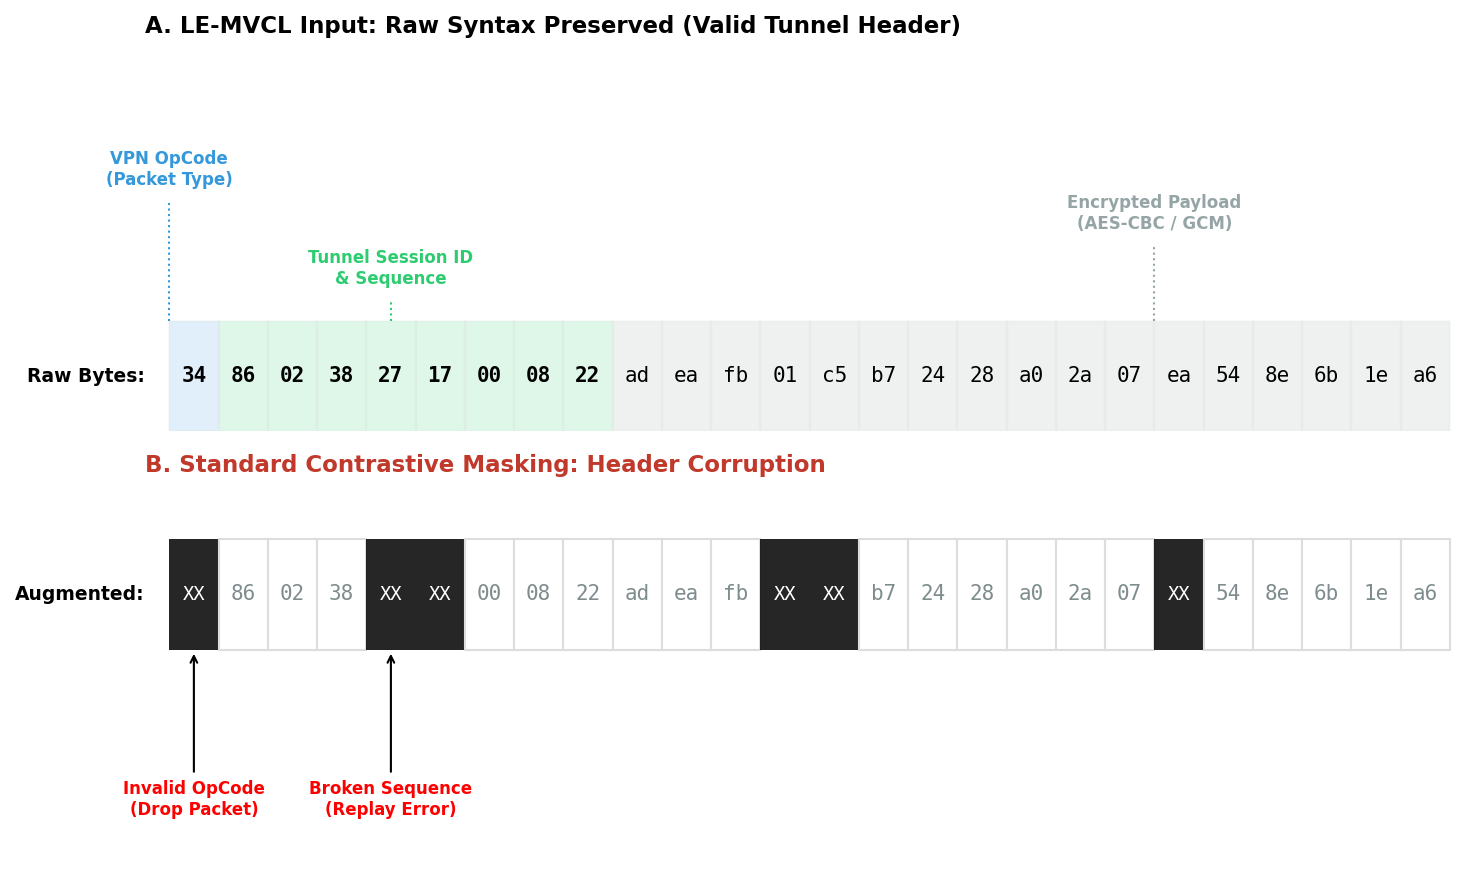
\includegraphics[width=\linewidth]{img/vpn_syntax_destruction.png}
    \caption{Impact of Symmetric Masking on Encrypted VPN Traffic. 
    Visualized using a real OpenVPN UDP packet from the ISCXVPN2016 dataset. 
    (A) LE-MVCL Input: The raw byte sequence is preserved, maintaining the validity of the outer VPN header (OpCode \texttt{0x1D}) and Sequence ID. 
    (B) Symmetric Masking: Random byte masking (standard in SimCLR) corrupts critical tunnel fields. Masking the \textit{OpCode} renders the packet protocol-invalid, while masking the \textit{Sequence ID} creates artifacts resembling replay attacks. This forces the encoder to learn from logically broken data.}
    \label{fig:vpn_syntax}
\end{figure}

Another limitation of existing SSL-based traffic analysis methods is their inability to exploit the inherent multi-view nature of network flows. Encrypted traffic simultaneously exhibits low-level payload structures and high-level statistical patterns, such as burst behavior, packet inter-arrival dynamics, and spectral characteristics. Many existing frameworks focus primarily on a single representation or treat multiple modalities through symmetric augmentation, thereby underutilizing the complementary information available across different traffic views.

To address these limitations, LE-MVCL introduces an \textit{Asymmetric Multi-View Pre-training} strategy that explicitly models the dual nature of encrypted traffic. Instead of generating artificial augmentations from a single modality, the framework aligns two complementary representations of the same flow. A 1D-CNN encoder processes the raw payload bytes, while a multilayer perceptron (MLP) processes global flow-level statistical features. The statistical representation acts as a semantic guide, encouraging the payload encoder to learn embeddings that correlate with stable behavioral patterns of the traffic flow. This asymmetric design enables the model to capture higher-level protocol semantics without requiring manual labels or syntactically destructive augmentations.

In addition to representation learning, another critical design consideration in encrypted traffic classification is the fusion of heterogeneous features. Several recent studies have explored multimodal architectures that combine payload-based features with statistical descriptors. Frameworks such as Deep-Full-Range (DFR) \cite{zeng2019deep} and related approaches \cite{liu2024adaptive} typically employ deep fusion mechanisms, where multiple feature modalities are first projected into a shared latent space through neural encoders before classification. Although this strategy allows joint representation learning, it may inadvertently compress fine-grained statistical signals. Metrics such as precise packet inter-arrival intervals, burst patterns, or spectral characteristics can become smoothed or distorted when passed through multiple nonlinear transformations, potentially reducing their discriminative value for distinguishing closely related applications.

To mitigate this issue, LE-MVCL adopts a \textit{Hybrid Late-Fusion} architecture. Instead of projecting all modalities into a shared deep latent space, the semantic embeddings learned from the payload encoder are concatenated directly with raw normalized statistical features, including Alpha, Beta, Gamma, and FFT-based spectral descriptors. This design preserves the high-resolution statistical information while still benefiting from the semantic abstraction learned through deep representation learning. As a result, the final classifier can leverage both the expressive capability of deep embeddings and the precise discriminative power of handcrafted statistical features, leading to improved performance in fine-grained encrypted application classification.





% \section{Related Work}
% \label{sec:related_work}

% \begin{table*}[htbp]
% \caption{Comparison of LE-MVCL with State-of-the-Art Frameworks}
% \label{tab:rw_comparison}
% \centering
% \begin{tabular}{l c c c c}
% \hline
% \textbf{Framework} & \textbf{Learning Paradigm} & \textbf{Pre-training Strategy} & \textbf{Fusion Type} & \textbf{Label Efficiency} \\
% \hline
% Deep Packet \cite{lotfollahi2020deep} & Supervised & None & None (Payload Only) & Low \\
% DFR \cite{zeng2019deep} & Supervised & None & Deep / Latent & Low \\
% Flow-GNN \cite{huoh2022flow} & Supervised & None & Graph + Flow & Medium \\
% Generic SSL (SimCLR-Net) & Self-Supervised & Symmetric (Augmentations) & None & Medium \\
% \textbf{LE-MVCL (Ours)} & \textbf{Semi-Supervised} & \textbf{Asymmetric (Payload $\leftrightarrow$ Stats)} & \textbf{Hybrid Late-Fusion} & \textbf{High} \\
% \hline
% \end{tabular}
% \end{table*}

% The classification of encrypted traffic has undergone a significant paradigm shift, evolving from port-based heuristics to sophisticated Deep Learning (DL) architectures. However, the field currently faces dual challenges: the prohibitive cost of acquiring labeled datasets and the technical difficulty of effectively fusing heterogeneous traffic views. In this section, we situate the proposed LE-MVCL framework within the broader landscape of supervised deep learning, contrastive representation learning, and multimodal fusion strategies.

% \subsection{Supervised Deep Learning and the Label Scarcity Bottleneck}
% With the obsolescence of port-based classification and the decreasing efficacy of traditional statistical machine learning, Deep Learning has emerged as the dominant paradigm for encrypted traffic analysis. Pioneering works by Wang et al. \cite{wang2017end} and Lotfollahi et al. \cite{lotfollahi2020deep} demonstrated that 1D-Convolutional Neural Networks (1D-CNNs) and Stacked Autoencoders (SAE) could automatically learn feature hierarchies from raw packet bytes, effectively treating network traffic analysis as a sequence modeling task akin to Natural Language Processing. Subsequent research has expanded this capability by incorporating Long Short-Term Memory (LSTM) networks \cite{yao2019identification} to capture temporal dependencies and Graph Neural Networks (GNN) \cite{huoh2022flow} to model the topological structure of traffic flows.

% Despite their high accuracy on benchmark datasets like ISCX-VPN-2016, these supervised models are fundamentally constrained by their reliance on massive, fully labeled datasets. In realistic operational environments, such as Security Operations Centers (SOCs), acquiring ground-truth labels for encrypted tunnels is a labor-intensive and costly process. Consequently, standard supervised architectures often suffer from severe performance degradation in low-resource settings. This limitation underscores the critical need for label-efficient frameworks capable of learning robust representations from the vast amounts of unlabeled traffic available in production networks.

% \subsection{From Symmetric to Asymmetric Contrastive Learning}
% To address the label scarcity problem, Self-Supervised Learning (SSL) has gained traction within the networking community. Techniques originally developed for Computer Vision, such as SimCLR \cite{chen2020simple}, have been adapted to traffic analysis, typically employing a \textit{symmetric} contrastive learning approach. In these methods, a single encoder is trained to maximize the agreement between two augmented views of the same flow, generated via techniques like random packet masking or payload shuffling.

% We argue, however, that symmetric augmentation is suboptimal for encrypted tunnel traffic. Unlike images, where pixel noise is tolerable, randomly masking packet bytes can destroy the rigid syntax of encapsulation protocols (e.g., OpenVPN, IPsec). In a VPN context, the "payload" seen by the model begins with a delicate outer header containing Opcodes and Sequence IDs required for tunnel integrity.

% To illustrate this empirically, we visualize the impact of these augmentations on real OpenVPN traffic from the ISCXVPN2016 dataset in Fig. \ref{fig:vpn_syntax}.

% \begin{figure}[h]
%     \centering
%     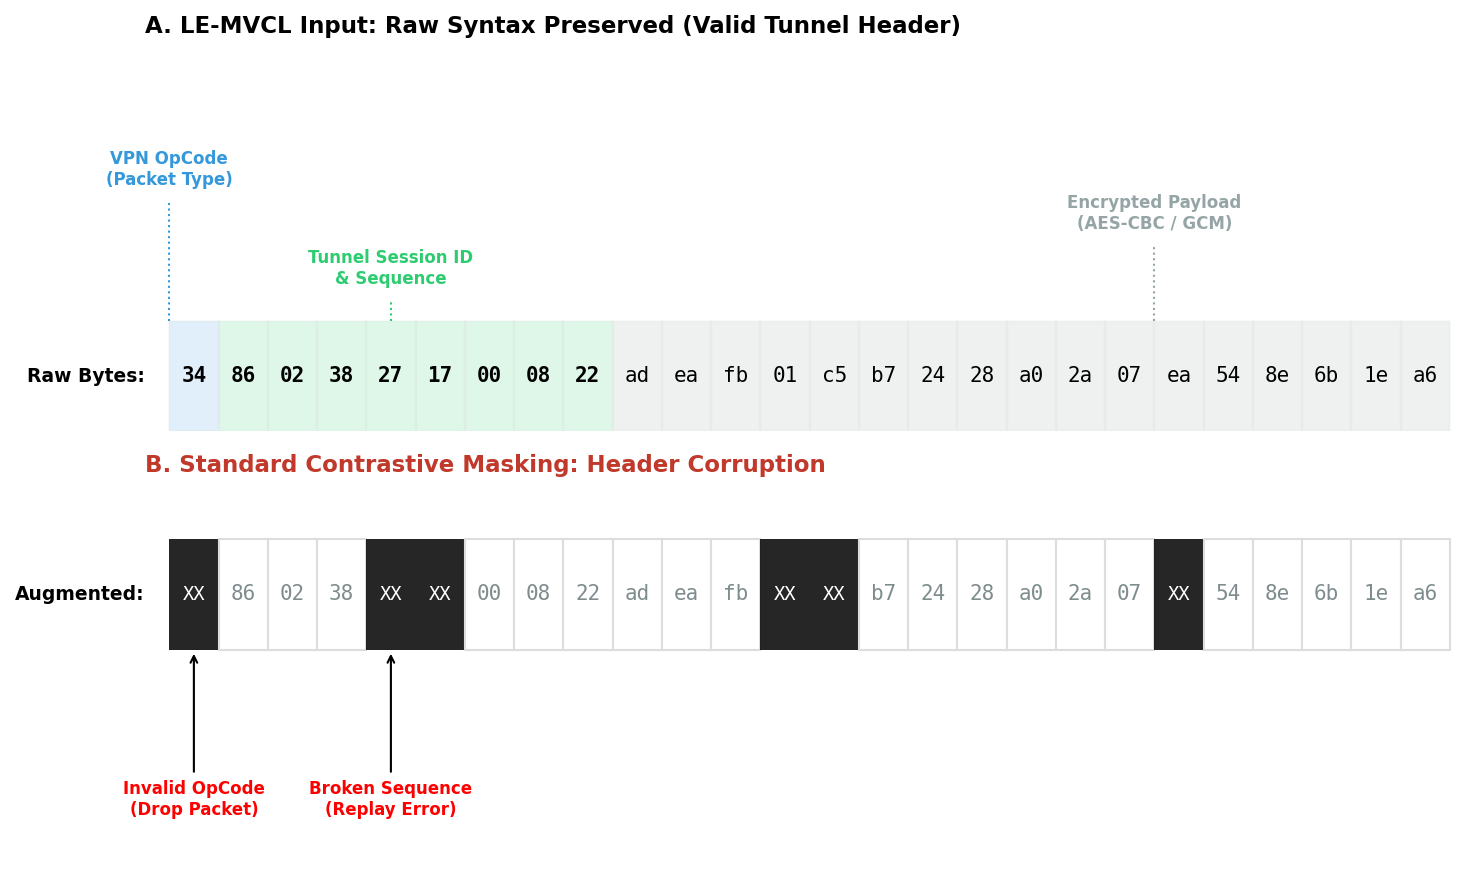
\includegraphics[width=\linewidth]{img/vpn_syntax_destruction.png}
%     \caption{Impact of Symmetric Masking on Encrypted VPN Traffic. 
%     Visualized using a real OpenVPN UDP packet from the ISCXVPN2016 dataset. 
%     (A) LE-MVCL Input: The raw byte sequence is preserved, maintaining the validity of the outer VPN header (OpCode \texttt{0x1D}) and Sequence ID. 
%     (B) Symmetric Masking: Random byte masking (standard in SimCLR) corrupts critical tunnel fields. Masking the \textit{OpCode} renders the packet protocol-invalid, while masking the \textit{Sequence ID} creates artifacts resembling replay attacks. This forces the encoder to learn from logically broken data.}
%     \label{fig:vpn_syntax}
% \end{figure}

% As demonstrated in Fig. \ref{fig:vpn_syntax}, a standard stochastic augmentation that blindly zeros out bytes has a high probability of corrupting the \textit{VPN OpCode} (identifying the packet type) or the \textit{Sequence Number} (critical for anti-replay logic). Unlike image cropping, which leaves the semantic object intact, this transformation renders the packet syntactically invalid—effectively asking the model to learn a representation for a "broken" tunnel state that never occurs in legitimate traffic. LE-MVCL (Fig. \ref{fig:vpn_syntax}A) addresses this by preserving the exact byte sequence and instead deriving the contrastive signal from the flow's global behavioral statistics.

% Furthermore, existing network SSL methods often ignore the inherent duality of traffic, failing to exploit the stable statistical properties of a flow to guide the learning of the more volatile payload representation. 

% In contrast, LE-MVCL introduces an \textit{Asymmetric Multi-View Pre-training} strategy. rather than relying on artificial augmentations, we align two distinct deep encoders: a 1D-CNN processing the raw payload and an MLP processing global flow statistics. By treating the robust statistical view as a "Semantic Guide," our approach forces the CNN to learn representations that correlate with global behavioral patterns, thereby capturing high-level protocol semantics without requiring explicit supervision.

% \subsection{Deep Embedding vs. Hybrid Late-Fusion}
% Recognizing that neither payload nor statistics alone suffice for fine-grained classification, recent literature has moved towards hybrid architectures. Frameworks such as "Deep-Full-Range" (DFR) \cite{zeng2019deep} and other multimodal approaches \cite{liu2024adaptive} typically employ a "Deep Fusion" strategy. In this paradigm, statistical features are passed through deep neural encoders and projected into a shared latent space alongside payload embeddings before classification.

% While conceptually appealing, we empirically identify a critical flaw in Deep Fusion regarding \textit{statistical compression}. Projecting precise metrics—such as exact inter-arrival times or spectral entropy peaks—through deep non-linear layers often "smooths out" the granular anomalies necessary to distinguish between isotocol services (e.g., distinguishing a Skype voice call from a Hangouts voice call). 

% To overcome this, LE-MVCL adopts a \textit{Hybrid Late-Fusion} architecture. Instead of fusing abstract latent vectors, we concatenate the learned semantic embeddings from the CNN directly with the \textit{raw, normalized} statistical features (Alpha, Beta, Gamma, FFT). This strategy ensures that the granular precision of the statistical view is preserved intact for the final decision boundary, enabling superior performance in fine-grained application classification where traditional deep fusion models often fail.